\documentclass[11pt]{article}

\usepackage{graphicx}
\usepackage{float}
\usepackage{listings}
\usepackage{amsfonts} 
\usepackage{amsmath}
\usepackage{amssymb}
\usepackage{placeins}
\usepackage[dvipsnames]{xcolor}

\usepackage[no-math]{fontspec} 
\setmainfont{Times New Roman}

\usepackage{hyperref}
\hypersetup{
    colorlinks=true,
    linkcolor=blue,
    filecolor=magenta,      
    urlcolor=cyan,
}

\definecolor{commentgreen}{rgb}{0.0, 0.5, 0.0}

\lstset{
  language=C,
  basicstyle=\footnotesize\ttfamily,
  numbers=left,           
  numberstyle=\tiny,       
  tabsize=5,                 
  extendedchars=true,         
  breaklines=true,
  commentstyle = \color{commentgreen},
  keywordstyle=\color{blue}\textbf,           
  stringstyle=\color{white}\ttfamily,
  showspaces=false,       
  showtabs=false,           
  showstringspaces=false,
  morekeywords={procedure, foreach, in}
}

\newcommand{\classname}[1]{\textit{\textbf{#1}}}
\newcommand{\varname}[1]{\underline{\textit{#1}}}
\newcommand{\funcname}[1]{\textit{#1}}

\title{ICS2211 Assignment}
\author{Lorenzo Catania, Malcolm Grech, Francesco Borg Bonello (Team \#8, life below water)}

\begin{document}

\maketitle

{
  \hypersetup{linkcolor=black}
  \tableofcontents
}

\section{Introduction}
\subsection{Game concept}
The presented project is a simil-arcade game called \textbf{Deep Blue}, set in a fictionary submarine world where fishes became so used to the garbage dumped in the ocean that they genetically mutated and started eating it.
You embody a scuba diver that has to collect as much rubbish as possible while being chased by mutant sea creatures.

\subsection{Game mechanics}
The game is a side-scroller runner where the world is discovered from left to right, with the camera moving accordingly.
The player has to collect as much garbage items (represented by cans, plastic bags, plastic bottles etc...) to increase its score.
Foes are spawned and will start patrolling different areas of the screen. If the player stays for a consistent time close enough to an enemy then it starts chasing and attacking the character. The player has no way to counterattack, its aim is to run away from fishes (they'll disappear completely after falling out of the left side of the camera).

The player must also take care of the oxygen available, that goes down while being underwater and can be recharged going back to the surface level. The oxygen drops faster based on the depth the character is on.
If the oxygen finishes, the player starts losing health.

It's possible to find some power-ups on the map or into trash items.
Those are useful to heal, recover oxygen or permanently increase the character's speed to make it easier to run away from enemies.

The environment is procedurally generated, meaning that each game may be potentially infinite. Items, collectables and enemies are spawned randomly on the right and are automatically garbage-collected when falling over the left of the screen.
The enemies strength grows over time and there's a little chance that an enemy evolves to a more dangerous kind of organism.

\section{Software architecture}
\subsection{Development environment}
The game has been developed using Unity3D 2018.4.13f and the game has been tested on both Windows and GNU/Linux operating systems. No specific versioning control software has been used, but it's possible to reconstruct a rough history of the code because each proposed change was packaged into a Unity Package and imported by the rest of the team after it was tested accurately.

\subsection{Components}
\subsubsection{Level generation}
The LevelGenerator is responsible for spawning collectables and in general any neutral entity the player can interact with.
It contains a list of prefabs with the respective probability of spawning and the range of coordinates they can appear into.
The level generation happens on an area placed on the right side of the camera that's still not visible to the player.
This area is splitted into tiles of fixed size and it's periodically filled with entities that are then attached to the root node of the scene so they can shift on the left and interact with the current game environment. Two entities spawned in the same update can't appear in near tiles to guarantee world variety.
Note that enemies could be spawned by level generator, but they're not in the final version of the game because a more dynamic way of evolving has been preferred. In fact, game objects spawned by level generator are initialized in-place and just deallocated when their cycle of life finishes. This approach doesn't affect performances for simple objects, but may limit the versatility of highly "intelligent" ones like enemies.

\begin{figure}[H]
  \centering
  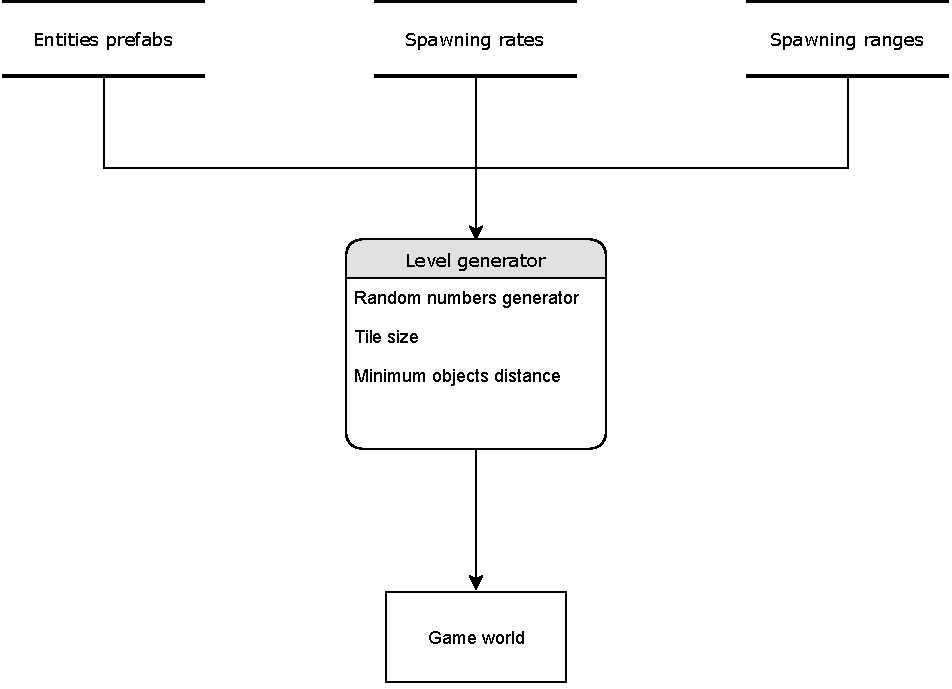
\includegraphics[width=1.0\textwidth]{figures/level_generator}
  \caption{Level generation data flow}
\end{figure}

\subsubsection{Camera movement control}
The CameraController component handles the main camera movement and the appearance of visual details in the scene.

The camera smoothly follows the player movement, but it's clamped on the vertical axis to avoid showing the void behind the background sprite. The camera moves slightly faster on the horizontal axis based on how close is the player to the right bound of the screen.

As the player object actually moves in the scene world, the background image must be continously shown and moved towards, without allowing the user to notice the loop and break the magic.

Two seamless background textures are loaded and put side by side. When the leftmost one remains out of camera visual, it's translated on the right of the other and so on.
Doing so the player will never see the void behind the background and performances won't be affected too much as the only operation done is a casual translation.

\begin{figure}[H]
  \centering
  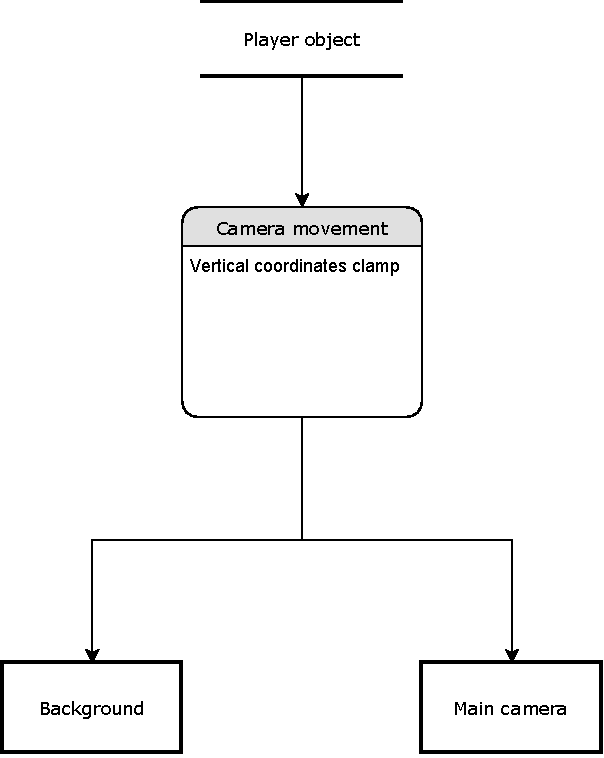
\includegraphics[width=0.8\textwidth]{figures/camera_controller}
  \caption{Camera control data flow}
\end{figure}

\subsubsection{Player control}
The player object is controlled using the mouse. The movement is smoothed based on how far is the mouse pointer and the rotation is not sudden as well to simulate a visual underwater physics effect. Furthermore, the head movement is faster than the body movement and tends to follow the mouse pointer much faster to give a better idea of where the player will go.

Player's health and oxygen values are handled by a script as well, mainly to determine the game over. External entities interactions (enemies, collectables etc...) may change those values as well.
The player position is checked on every update loop to determine whenever oxygen is gained or spent based on the depth (represented by its position in the Y axis).

Raycasting is used all around the player object to see if any collectable is present and in case there is to pick it up.

\begin{figure}[H]
  \centering
  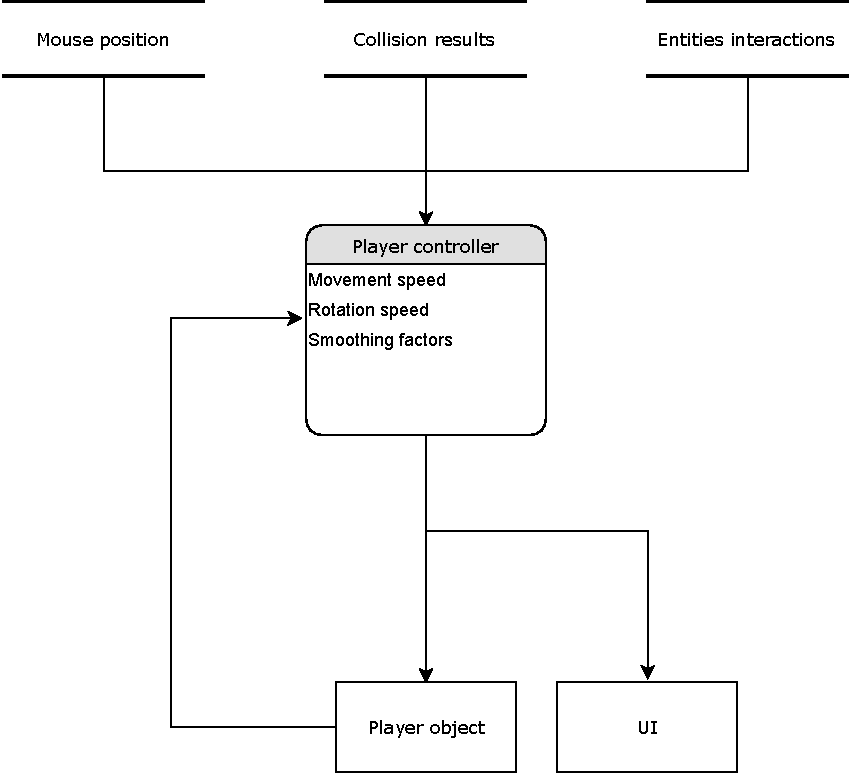
\includegraphics[width=1.0\textwidth]{figures/player_controller}
  \caption{Player control data flow}
\end{figure}

The backward arrow between the player object and its controller represents the usage of current player data (for example, the position) to compute what the values should be present in the next step.

\subsubsection{Entities garbage collection}
A "death wall" object is placed on the left of the screen and it moves following the camera. It has a trigger that collides with all the game objects (expect the background sprites). Each time an object is far enough from the user's point of view it gets deleted or sent back to its relative pool to optimize memory usage and clean up the scene from useless objects that shouldn't be rendered anymore.

\subsubsection{Game state and UI}
In the current version, the game state is given only by the score. A \textit{ScoreManager} is used to take track of its value and to update the score's label on the GUI.

Menus are composed by simple buttons that interact with a \textit{ButtonHandler}, calling different function based on what action must be executed (most of the time they load a different scene).
In-game user interface is made of icons and sliders or texts that represents the player stats and the current user score. They're updated by controller as well. A more in-depth analysis on the menu system is contained in the next section.

\subsubsection{Menu interface}
The game menu had been designed with functions that are global throughout all scenes, such as the ability to go to the settings when pressing escape/ pausing, and initially a single sound track until it was decided to have different sounds per scene. This was done by the player loading into a master scene to load these functions, then strait to their mainMenu scene. 
With an option of 3 buttons, the player may begin playing, go to the setting scene, were sound may be adjusted, or terminate the program. When pressing ‘Escape’ or ‘Enter’ at any point while in the main menu or in gameplay to load the settings scene, and press one of them again to return to the previous scene, or do so by means of another button. 
When in the settings scene, the player may adjust the volume of the sound track, and was planned to pause the gameplay should the player have been in gameplay mode. The pause feature however was not successfully implemented entirely.

\begin{figure}[H]
  \centering
  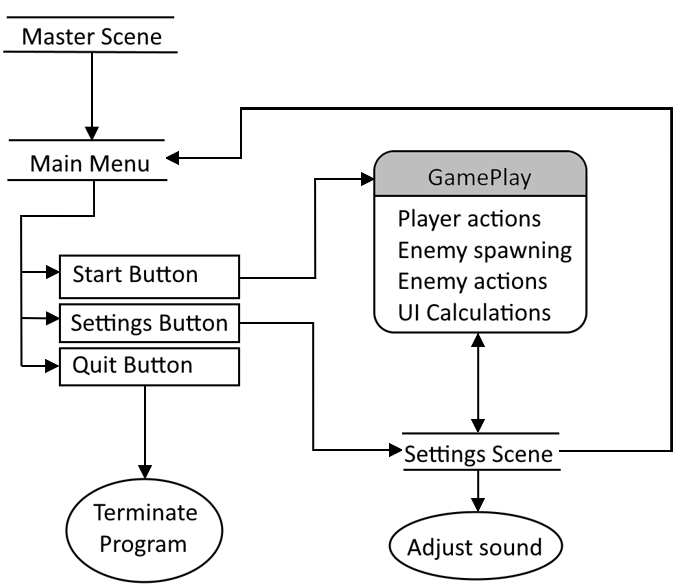
\includegraphics[width=0.6\textwidth]{figures/menu_system}
  \caption{Menus data flow}
\end{figure}

\subsubsection{Enemies spawning}
Model used to spawn enemies in the game world is unique and tuned specifically for gradually increasing the match difficulty.
It's based on a genetic algorithm, applied to a pool of pre-instantiated enemy objects that are partially destroyed and initialized again during the breeding phase.

Enemies in the pool are breeded periodically, while a new enemy is popped out from the pool and spawned in the world once in a while. Note that enemies currently present in the scene are not involved in breeding, so the process is completely invisible to the user.

Different kind of enemies can be encountered while playing and the variety is guaranteed by mutations during reproduction on fishes, meaning that a child may mutate to a different species instead of inherating its genes from the parents. The chance of encountering weaker species decreases over time.

The approach used to breed enemies is described in details in the next section.

\begin{figure}[H]
  \centering
  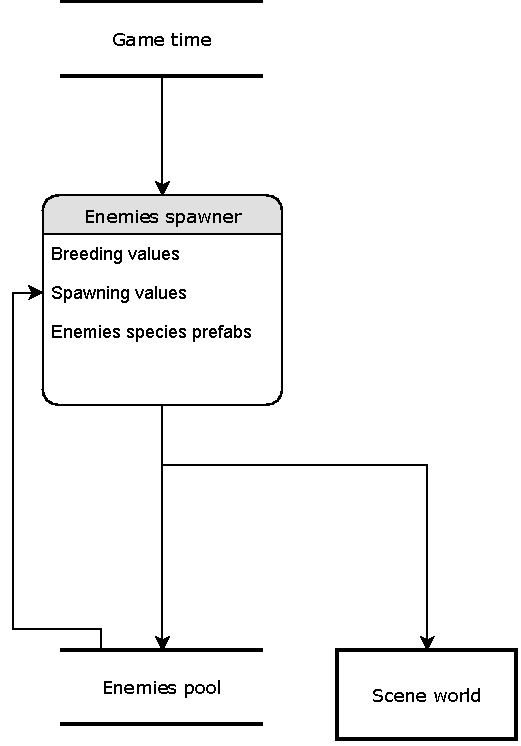
\includegraphics[width=0.6\textwidth]{figures/enemies_spawner}
  \caption{Enemies spawner data flow}
\end{figure}

\section{Artificial Intelligence features}
\subsection{Enemies behaviour state machine}
The enemies behaviour is traced by a simple finite state machine that contains two states: \classname{patrolling} and \classname{attack}.

\begin{figure}[H]
  \centering
  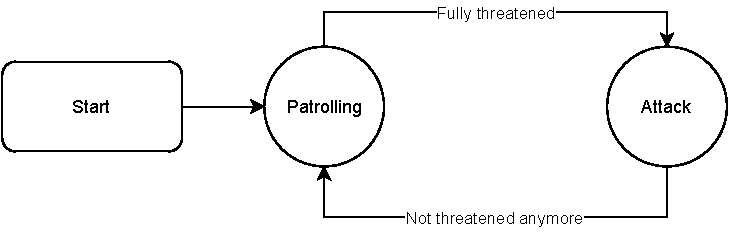
\includegraphics[width=0.6\textwidth]{figures/enemy_behaviour_states}
  \caption{Enemy behaviour state machine}
\end{figure}

Transitions between those two states are triggered by a single variable \varname{threat}. The threat level increases and decreases based on how far the player is from an enemy and for how much time.

Threating is based on a fuzzy system, defined by the \varname{threat} value itself, \varname{onAlertThreshold} and \varname{attackThreshold}.

\begin{figure}[H]
  \centering
  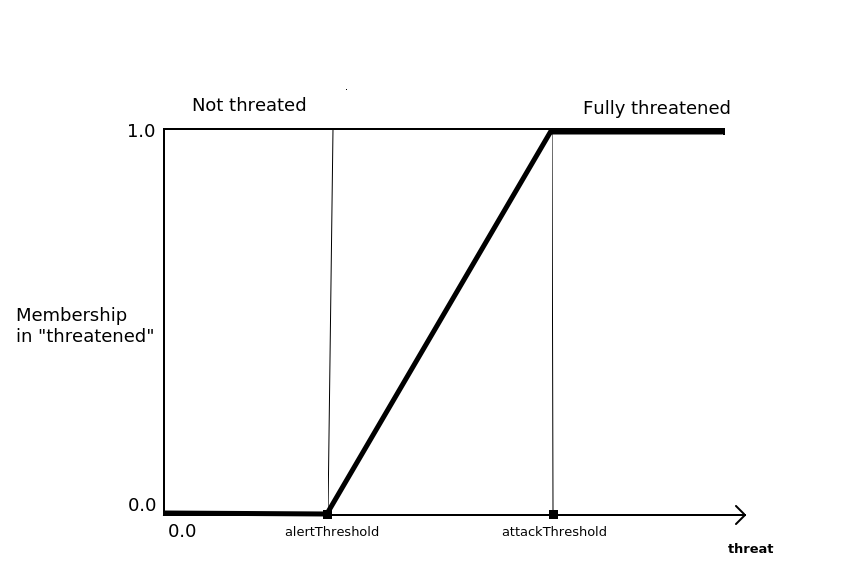
\includegraphics[width=0.8\textwidth]{figures/threat_graph}
  \caption{Threatening evaluation graph}
\end{figure}

As the \varname{threat} value grows, the enemy is first on guard and then starts attacking. When \varname{threat} value goes down, the enemy stops chasing and keeps patrolling again.

Note that if $alertThreshold < threat < attackThreshold$ the enemy's behaviour state doesn't change. While in this level, the enemy keeps active as before until one of the thresholds is hit.

\FloatBarrier

\begin{figure}
  \begin{lstlisting}
  procedure PatrolB positionehaviourUpdate():
      // Moves randomly around the current position
      PatrolArea() 

      if threat > attackThreshold:
        SetState(Attack)
  \end{lstlisting}
  \caption{Enemy patrolling state update pseudocode}
\end{figure}

\begin{figure}
  \begin{lstlisting}
    procedure AttackBehaviourUpdate():
      // Moves towards the player
      ChaseEntity(playerObject) 

      // If close enough to the player
      // attack him and reduce its HP
      if CloseTo(playerObject) and attackCooldown == 0: 
        Attack(playerObject)

      if threat < alertThreshold: 
        SetState(patrol)
  \end{lstlisting}
  \caption{Enemy attack state update pseudocode}
\end{figure}

\FloatBarrier

\subsection{Enemy evolution}
Enemies are supposed to get stronger as the game progresses.
To obtain that, enemies a fixed number of enemies with random stats is instatiated \textit{(default = 10)} and stored in an object pool before the actual game starts. The enemies in that pool are called \textit{offline} or resting enemies.

During the game, once in a while, an enemy is extracted from the pool and spawned on the game field. Enemies present in the game world are called \textit{online} or spawned enemies. After those enemies are taken out of the game scene they go back to the offline pool.

This trick is already useful to improve performances as game objects are less likely to be created from scratch during the game, but the most interesting thing is that we can modify the offline enemies without any visible interruption of the gameplay.

\subsubsection{Stats}
Each enemy entity has different stats that evolve over time:

\begin{itemize}
  \item \textbf{Patrol speed} (\textit{patrolSpeed}): Movement speed while patrolling
  \item \textbf{Patrol zone size} (\textit{patrolZoneSize}): Size of the patrol zone
  \item \textbf{Patrol threat range} (\textit{patrolThreatRange}): Range from where the enemy is threatened by player's presence
  \item \textbf{Patrol threat growth} (\textit{patrolThreatGrowth}): The speed at which the threat value grows while patrolling
  \item \textbf{Patrol threat decay} (\textit{patrolThreatDecay}): The speed at which the threat value decreases while patrolling

  \item \textbf{Chasing speed} (\textit{chasingSpeed}): Movement speed while chasing the player
  \item \textbf{Attack range} (\textit{attackRange}): The minimum range to attack the player
  \item \textbf{Maximum chase range} (\textit{maximumChaseRange}): The maximum distance after which the enemy stops chasing the player
  \item \textbf{Attack damage} (\textit{attackDamage}): Damage dealt to the player after an attack
  \item \textbf{Maximum attack cooldown} (\textit{maxAttackCooldown}): The cooldown time between two consecutive attacks
  \item \textbf{Attack threat growth} (\textit{attackThreatGrowth}): The speed at which the threat value grows while attacking
  \item \textbf{Attack threat decay} (\textit{attackThreatDecay}): The speed at which the threat value decreases while attacking
\end{itemize}

Those values are considered the \textit{genes} of the enemy as they define how \textit{strong} an enemy is. The \textit{strength} of an enemy is based on part of its stats and is evaluated using this formula:

\begin{gather*}
  strength(foe) =
    foe.patrolSpeed + \\
    foe.patrolZoneSize + \\
    foe.patrolThreatRange + \\
    foe.hasingSpeed + \\
    foe.attackRange + \\
    foe.maximumChaseRange + \\
    \frac{foe.attackDamage}{5} + \\
    \frac{2}{foe.maxAttackCooldown}
\end{gather*}

\pagebreak

\subsubsection{Breeding}
The \textit{breeding} phase involves two different enemies and produces a child which stats are the result of taking the best stats of both parents and mixing them together.
This approach ensures that a child will always be at least as strong as the parents, making the game rapidly more difficult in the progress.

\begin{figure}[H]
  \begin{lstlisting}
  procedure Breed(parent1, parent2):
    child = CreateEmptyEnemy()

    if strength(parent1) > strength(parent2):
      child.kind = parent1.kind
    else:
      child.kind = parent2.kind

    foreach stat_var in child:
      child.stat_var = max(parent1.stat_var, parent2.stat_var)

    return child 
  \end{lstlisting}
  \caption{Breeding procedure pseudocode}
\end{figure}

\subsubsection{Mutations}
There's always a chance that during breeding the child genes mutate, leading to a totally different result than what's expected.
When a child mutates, its kind and its genes are generated randomly again instead of being derived from the parents.
The kind is chosen from all possible kinds, but weaker kinds of foes stop spawning after a while to ensure that while the game progresses new types of enemies are present and that the difficulty doesn't decrease. 
The genes are initialized randomly like when the initial population is instantiated at the start of the game.

Note that a mutation doesn't assure that the resulting enemy will be stronger or equal to the parents, nor will be of a stronger kind. The trend of the strength of spawned enemies is not monotonic, but tends to grow over time.

\subsubsection{Genetic selection overview}
The genetic selection step is executed on fixed intervals of time and involves only offline enemies. As it replaces a consistent number of entities it requires the offline pool to be big enough, otherwise the step is skipped.

Enemies present in the pool are sorted by their strength and best worst pairs of enemies are popped out. Best enemies are breed to generate two new children, while worst two are destroyed and replaced with two brand new enemies of the weakest kind possible with randomly generated stats.

\begin{figure}[H]
  \begin{lstlisting}
  procedure GeneticSelectionStep():
    SortByStrength(offlineEnemies)

    topEnemy1 = PopFromTop(offlineEnemies)
    topEnemy2 = PopFromTop(offlineEnemies)

    worstEnemy1 = PopFromBottom(offlineEnemies)
    worstEnemy2 = PopFromBottom(offlineEnemies)

    // Breed top enemies
    // Note that mutations can occur in this phase on both
    // of the calls of Breed()
    Push(offlineEnemies, Breed(topEnemy1, topEnemy2))
    Push(offlineEnemies, Breed(topEnemy2, topEnemy1))

    // Replace worst enemies with new ones
    Push(offlineEnemies, GenerateNewEnemy())
    Push(offlineEnemies, GenerateNewEnemy())
  \end{lstlisting}
  \caption{Genetic selection step procedure pseudocode}
\end{figure}

Not all offline enemies are involved in breeding. Some remain in the pool as they are and will be involved in mating/replacing in subsequent steps.

It may be possible to create a bigger pool and use more pairs during genetics election. However, the simple approach shown above requires little computational power and still gives good results in terms of game progression.

\subsubsection{Literature references and further readings}

The enemy behaviour approach was highly inspired by the concepts of \textit{fuzzy logic} developed by Lofti Zadeh (1921-2017) and proposed as an application in its 1973 paper \textit{"Outline of a new approach to the analysis of complex systems and decision processes"} from \textit{IEEE Trans. Systems, Man and Cybernetics, 1973; 3: 28–44}. Although using a single variable doesn't express the full power of fuzzy systems, the results were good enough to not make the enemy behaviour more complex than what it is.

Enemy evolution algorithm is based on the theory of \textit{Genetic algorithms} by John Holland (1929-2015) during the '60s and extensively described in \textit{Adaptation in Natural and Artificial Systems (1975, MIT Press)}, which is considered the killer book on genetic algorithms. As the game theme is about mutations and species evolution, this approach was literally the first that came in mind while planning down the enemies system.

The level generation algorithm was inspired by the demonstration material from Week 9 of the course.

\section{Conclusions}
\subsection{Team role}
\subsubsection{Lorenzo Catania}
I've made my part on the game development as a game script programmer,gameplay designer and sound/FX and music composer.

\subsubsection{Malcolm Grech}
My role in the game development was as a mostly as a backend developer with some frontend jobs.

\subsection{Personal contributions}
\subsubsection{Lorenzo Catania}
I've designed and implemented the camera movement controller, the entities garbage collection and most of all the enemy spawning, evolution and behaviour.

I've partecipated in designing and tuning the level generation and the score system.

I've edited the FX sounds, but none of them was originally created by me.

I've also composed the menu background music, trivially titled \textit{Deep Blue menu song}.

\subsubsection{Malcolm Grech}
My contribution to the game development where:
Creating the Menu scene Management and button/scroller functionality.
A part in the creation of the player movement and camera controller.
Creating the level generation which was fine tuned with other later additions.

\subsection{Final thoughts}
\subsubsection{Lorenzo Catania}
I would like to say thanks to everyone that has permitted this beatiful experience, first of all my whole team that worked wonderfully without any stops during the 2 days of the jam. Thanks also to University of Malta and its lecturers for guiding me in its new experience, as well as GDG Malta, MITA and all of the organizers of the event. Thanks to the catering as well, that was pretty good throughout all the weekend.

\subsubsection{Malcolm Grech}
The experience of my first gameJam was an extremely satisfying and enjoyable one. Having been allocated time to focus on creating a source of entertainment with a team of other capable creators was an honour. My only displeasures where my lack of connecting to my teammates, as my work was on occasion undermined and taken over. Though I had made significant contributions to the game development, I feel like I could have done better, and pushed more till the end as I plan to do in future Jams.

\end{document}